\section{Results}\label{sec:results}

In this section, we overview the performance results and the resource
utilization all the kernels implemented on GPU for face detection. 
Although, occupancy is not a direct measure of performance, it is important 
to have full occupancy for the GPU SMs. Based on the utilzation analysis done for all the kernels,

Table~\ref{table:util} shows the occupancy of each of the kernels. This includes the resgiters, 
shared memory and constant memory used for the kernels. As discussed in Section~\ref{sec:haar_optim}, 
relaxing the maximum resgiters used by thread is an optimization. We apply this optimzation and check for the 
occupancy of each kernel. 
However, this constarint can be relaxed only if all the threads in the thread block can accomodated with that register usage.
In our case, relaxing this constaint did not put a constaint on the threads that can be launched with each kernel.
We see that for \emph{RowScan Only} kernel the occupancy reduces due to this relaxation. However, the results of that kernel
show that it did not impact for the performance. 


\begin{figure*}
  \centering
  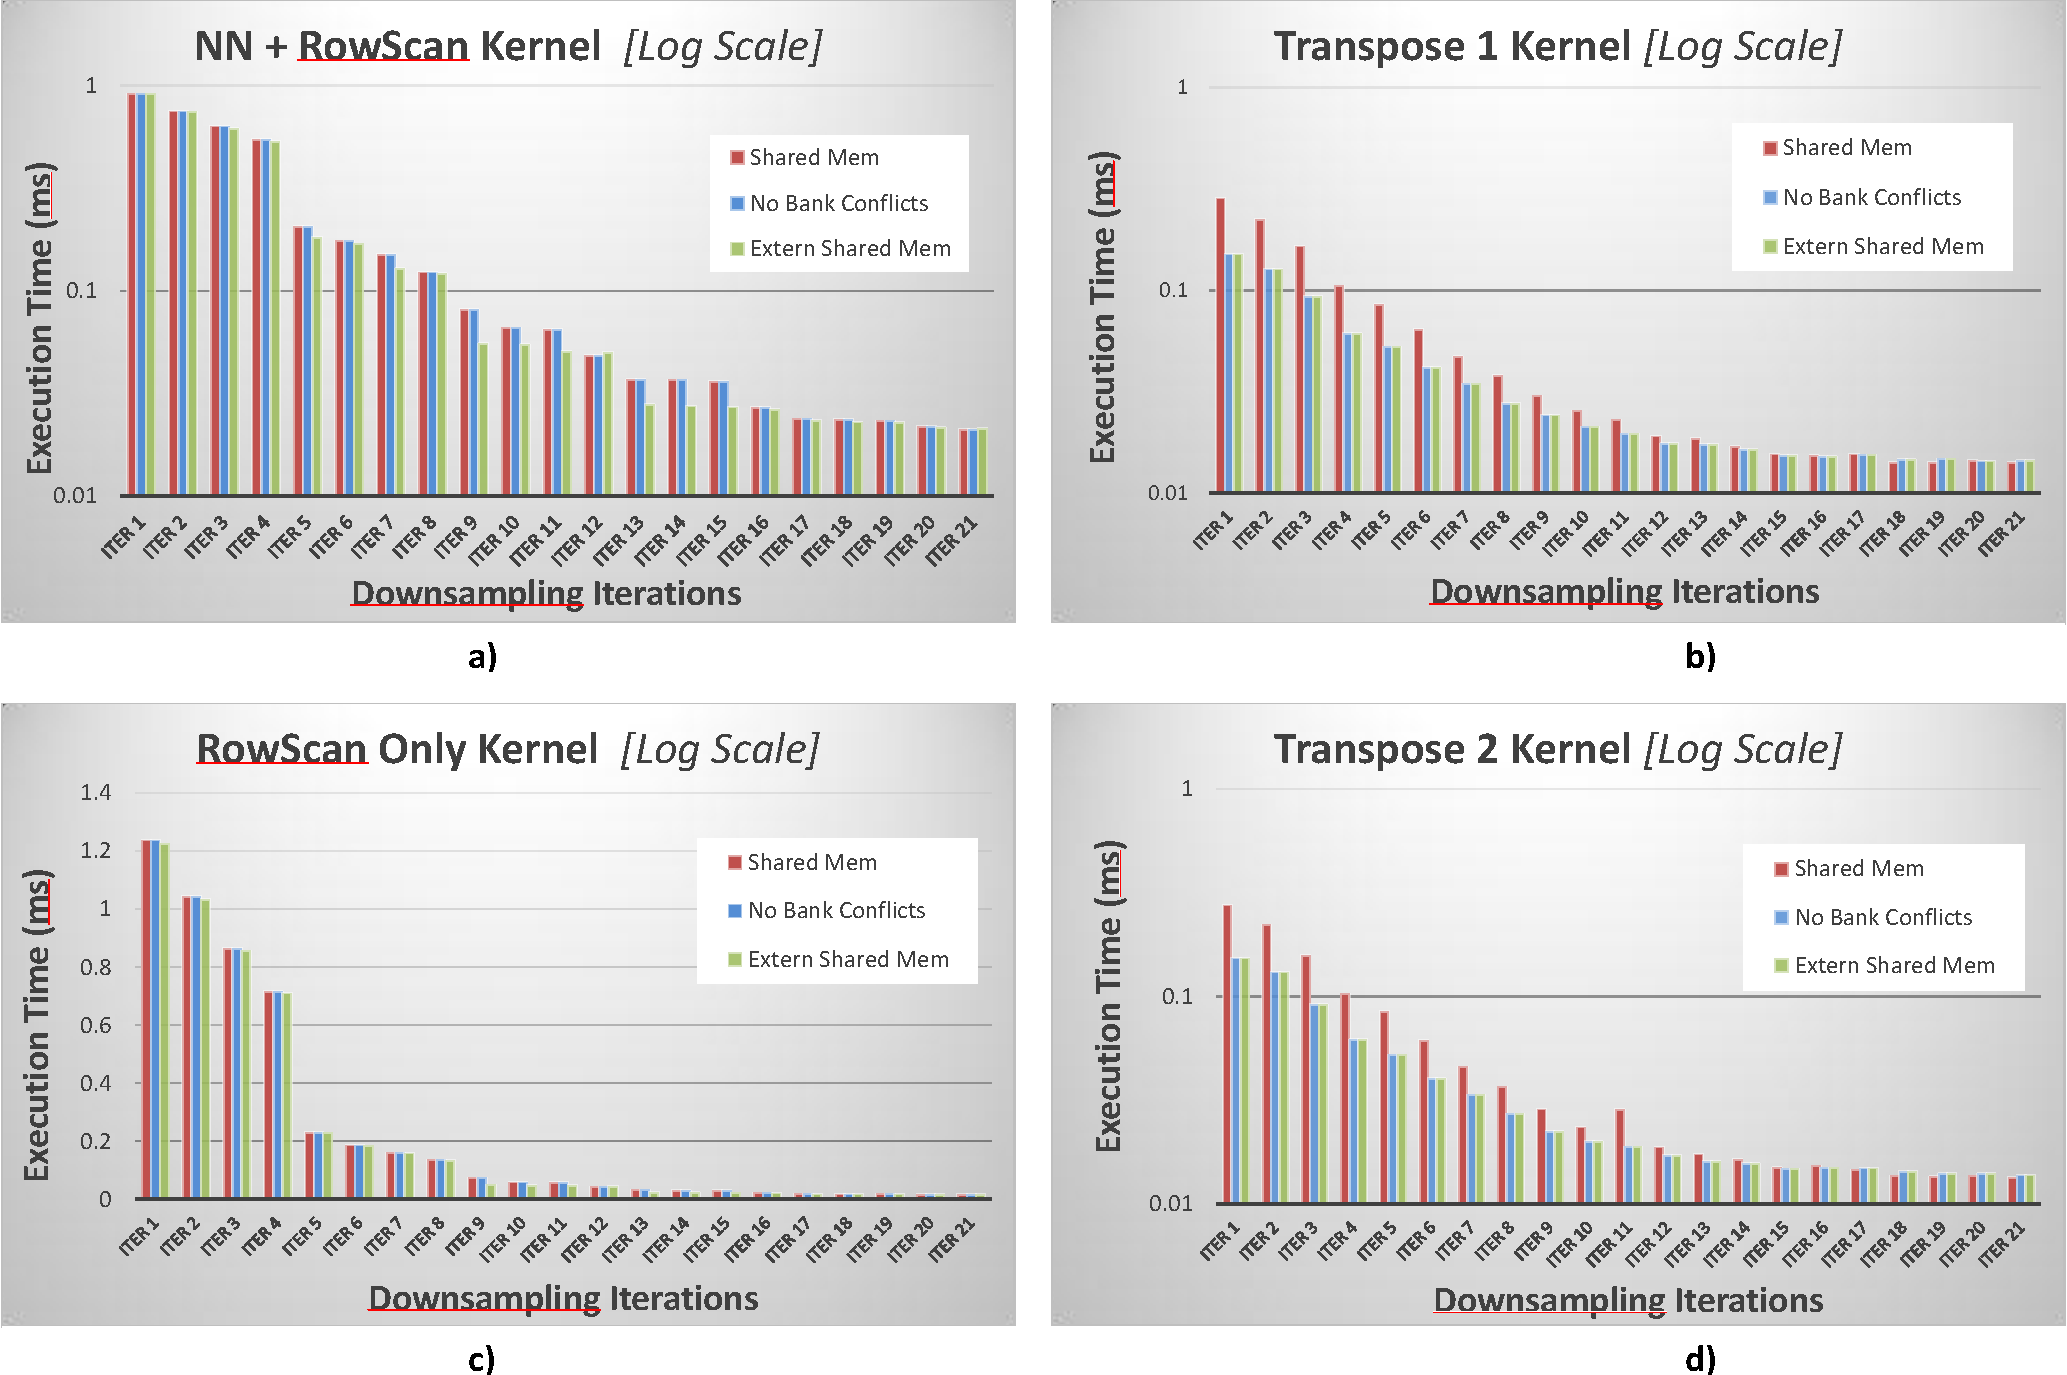
\includegraphics[width=\linewidth]{figs/nn_ii_kernels_crop.pdf}
  \caption{Performance of NN and II kernels; a) NN + RowScan; b) Transpose 1; c) RowScan Only; d) Transpose 2}
  \label{fig:nn_ii_kernels}
\end{figure*}

\vspace{0.1in}
\begin{figure*}[h]
  \centering
  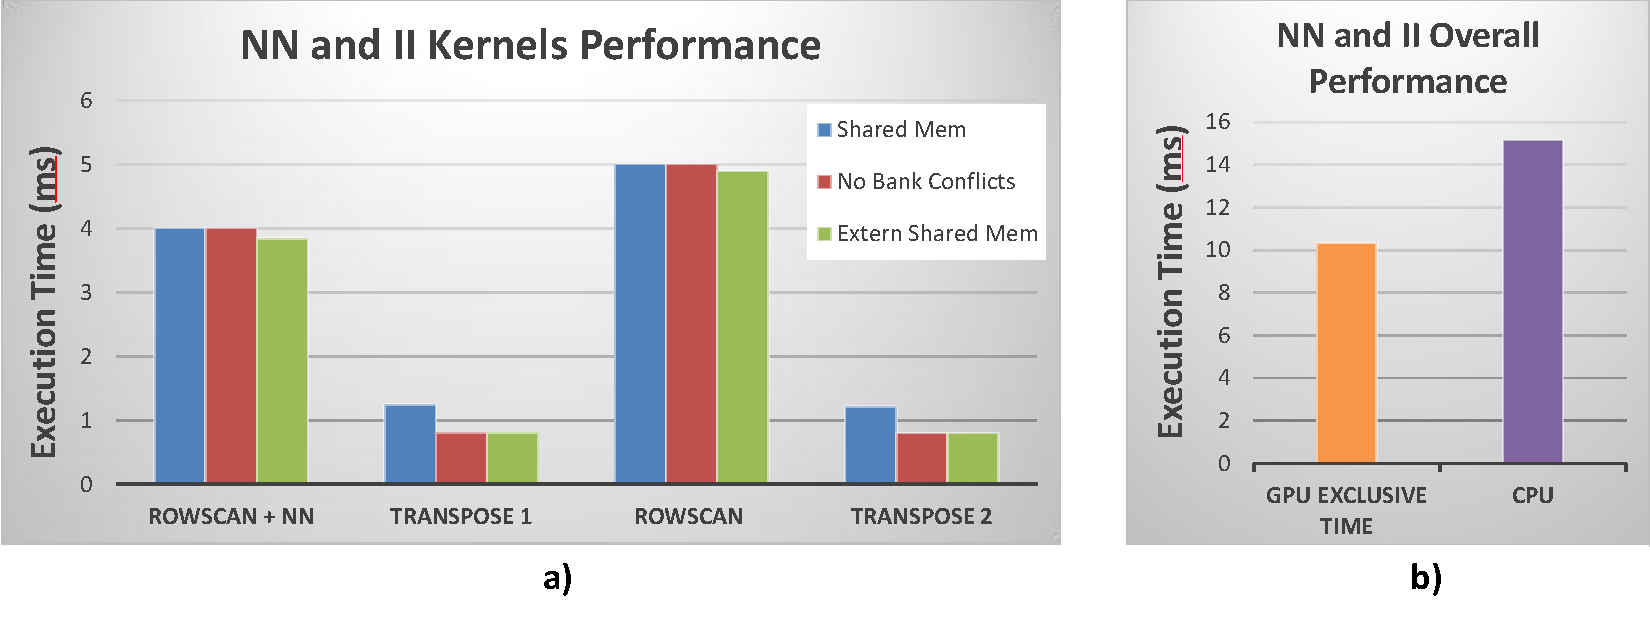
\includegraphics[width=0.9\linewidth]{figs/nn_ii_overall_crop.pdf}
  \caption{nn ii }
  \label{fig:nn_ii_overall}
\end{figure*}

\subsection{Performance of Nearest Neighbor and Integral Image Kernels}
Figure~\ref{fig:nn_ii_kernels} shows the performance of individual kernels of NN and II stage.
We apply the 3 optimizations discussed in Section~\ref{sec:nn_optim} here. Since, NN and II kernels 
contributed to only 3\% of the overall parallelization scope, we directly implemented the Shared mmeory version of the kernels
and that act as the baseline for NN and II kernels. When we applied the \emph{No bank conflicts} optimzation, only the \emph{Transpose 1}
and


\begin{figure*}[h]
  \centering
  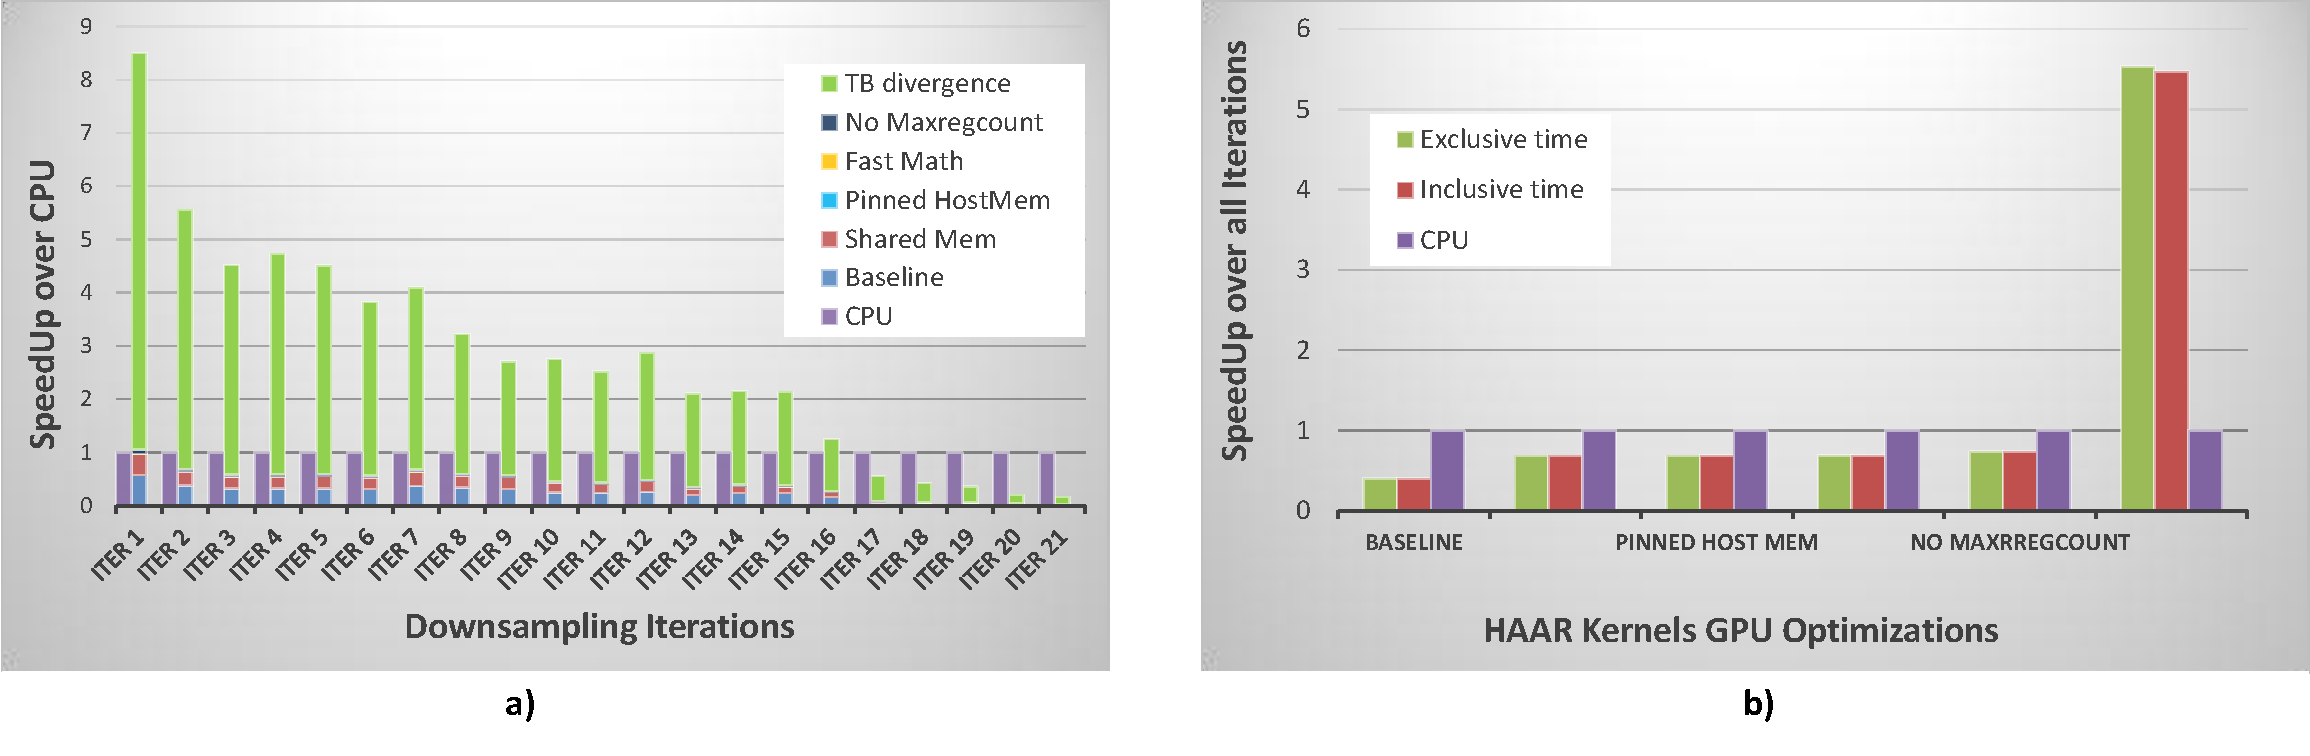
\includegraphics[width=\linewidth]{figs/haar_overall_crop.pdf}
  \caption{haar overall}
  \label{fig:haar_kernels}
\end{figure*}


\begin{figure}[h]
  \centering
  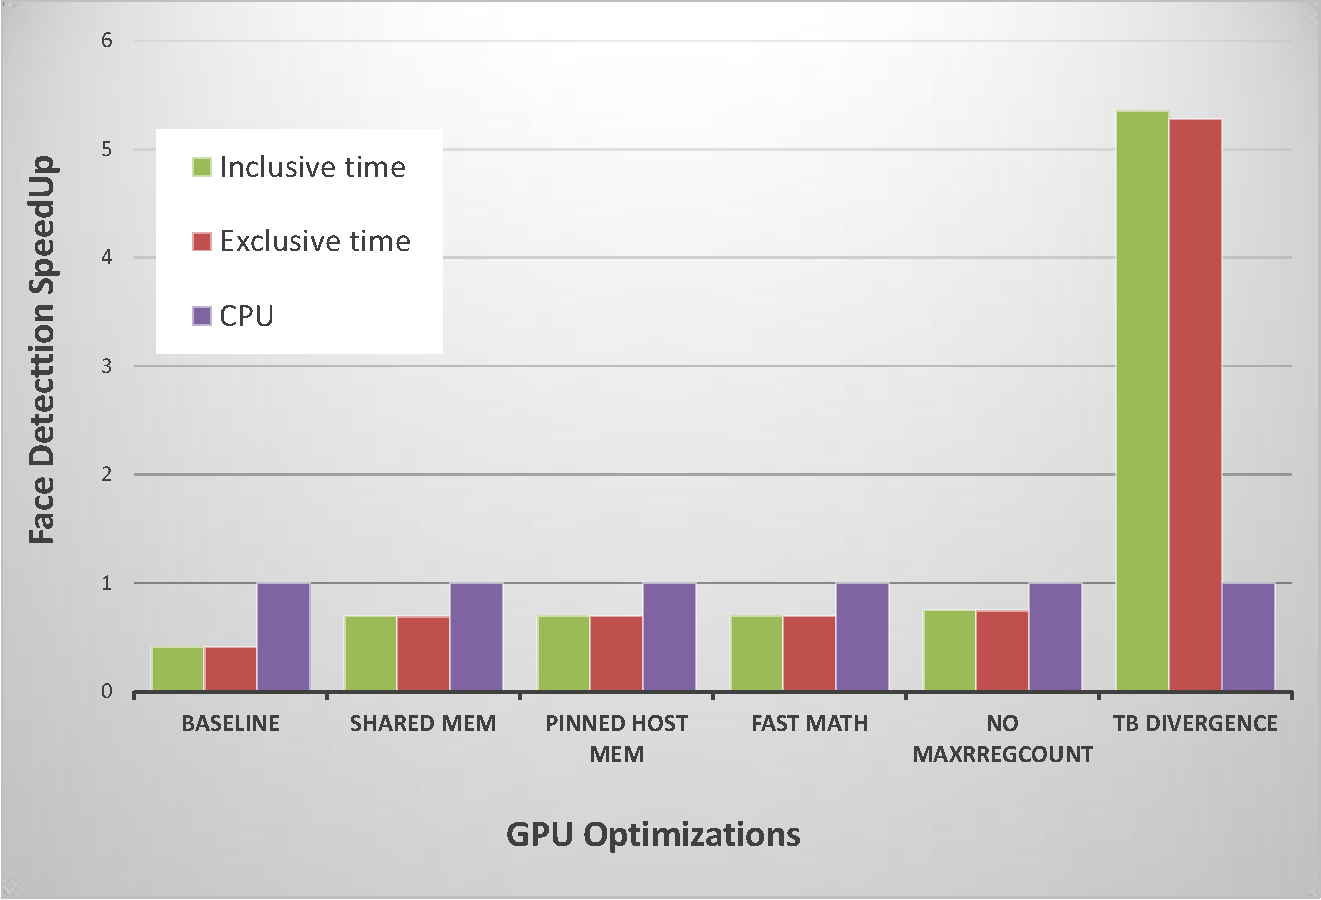
\includegraphics[width=\linewidth]{figs/gpu_overall_crop.pdf}
  \caption{gpu overall}
  \label{fig:haar_kernels}
\end{figure}


\begin{figure}[h]
  \centering
  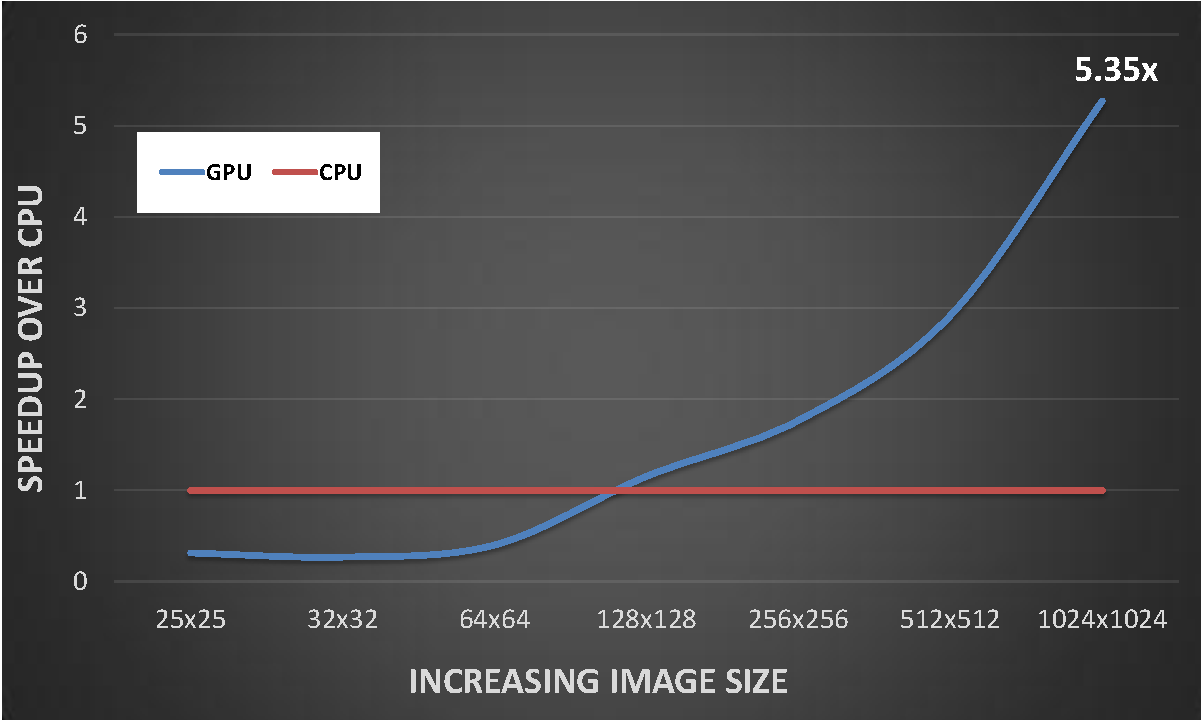
\includegraphics[width=\linewidth]{figs/image_size_crop.pdf}
  \caption{image sizes}
  \label{fig:haar_kernels}
\end{figure}


\begin{figure}[h]
  \centering
  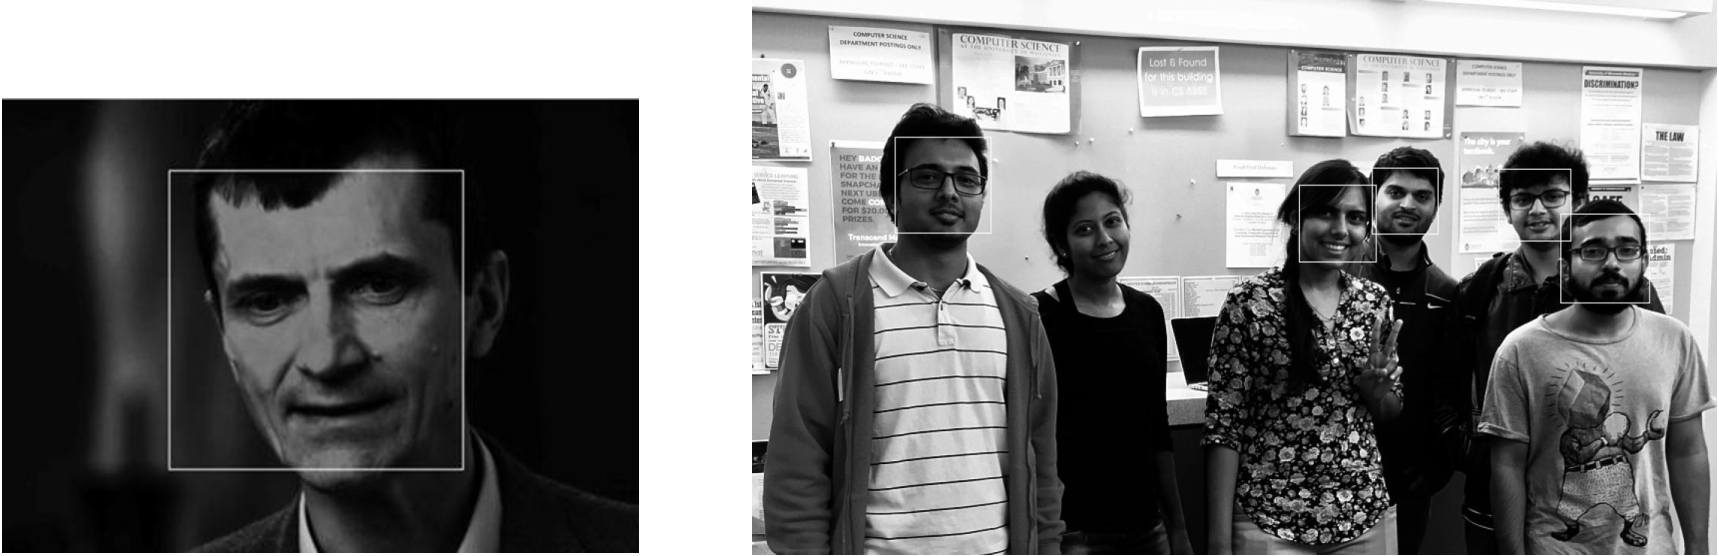
\includegraphics[width=\linewidth]{figs/face_detected_crop.pdf}
  \caption{image sizes}
  \label{fig:haar_kernels}
\end{figure}



